% Options for packages loaded elsewhere
\PassOptionsToPackage{unicode}{hyperref}
\PassOptionsToPackage{hyphens}{url}
\PassOptionsToPackage{dvipsnames,svgnames,x11names}{xcolor}
%
\documentclass[
]{memoir}
\usepackage{amsmath,amssymb}
\usepackage{lmodern}
\usepackage{iftex}
\ifPDFTeX
  \usepackage[T1]{fontenc}
  \usepackage[utf8]{inputenc}
  \usepackage{textcomp} % provide euro and other symbols
\else % if luatex or xetex
  \usepackage{unicode-math}
  \defaultfontfeatures{Scale=MatchLowercase}
  \defaultfontfeatures[\rmfamily]{Ligatures=TeX,Scale=1}
  \setmonofont[]{Inconsolata}
\fi
% Use upquote if available, for straight quotes in verbatim environments
\IfFileExists{upquote.sty}{\usepackage{upquote}}{}
\IfFileExists{microtype.sty}{% use microtype if available
  \usepackage[]{microtype}
  \UseMicrotypeSet[protrusion]{basicmath} % disable protrusion for tt fonts
}{}
\makeatletter
\@ifundefined{KOMAClassName}{% if non-KOMA class
  \IfFileExists{parskip.sty}{%
    \usepackage{parskip}
  }{% else
    \setlength{\parindent}{0pt}
    \setlength{\parskip}{6pt plus 2pt minus 1pt}}
}{% if KOMA class
  \KOMAoptions{parskip=half}}
\makeatother
\usepackage{xcolor}
\IfFileExists{xurl.sty}{\usepackage{xurl}}{} % add URL line breaks if available
\IfFileExists{bookmark.sty}{\usepackage{bookmark}}{\usepackage{hyperref}}
\hypersetup{
  pdftitle={Data Science per psicologi},
  pdfauthor={Corrado Caudek},
  colorlinks=true,
  linkcolor={Maroon},
  filecolor={Maroon},
  citecolor={Blue},
  urlcolor={Blue},
  pdfcreator={LaTeX via pandoc}}
\urlstyle{same} % disable monospaced font for URLs
\usepackage{longtable,booktabs,array}
\usepackage{calc} % for calculating minipage widths
% Correct order of tables after \paragraph or \subparagraph
\usepackage{etoolbox}
\makeatletter
\patchcmd\longtable{\par}{\if@noskipsec\mbox{}\fi\par}{}{}
\makeatother
% Allow footnotes in longtable head/foot
\IfFileExists{footnotehyper.sty}{\usepackage{footnotehyper}}{\usepackage{footnote}}
\makesavenoteenv{longtable}
\usepackage{graphicx}
\makeatletter
\def\maxwidth{\ifdim\Gin@nat@width>\linewidth\linewidth\else\Gin@nat@width\fi}
\def\maxheight{\ifdim\Gin@nat@height>\textheight\textheight\else\Gin@nat@height\fi}
\makeatother
% Scale images if necessary, so that they will not overflow the page
% margins by default, and it is still possible to overwrite the defaults
% using explicit options in \includegraphics[width, height, ...]{}
\setkeys{Gin}{width=\maxwidth,height=\maxheight,keepaspectratio}
% Set default figure placement to htbp
\makeatletter
\def\fps@figure{htbp}
\makeatother
\setlength{\emergencystretch}{3em} % prevent overfull lines
\providecommand{\tightlist}{%
  \setlength{\itemsep}{0pt}\setlength{\parskip}{0pt}}
\setcounter{secnumdepth}{5}
\chapterstyle{bianchi}

\usepackage{mathtools}
\usepackage[italian]{babel} 
\usepackage{booktabs}
\usepackage{hyperref}
\hypersetup{
  colorlinks=true
}
\usepackage[
  labelfont=bf, 
  font={small, it} 
]{caption} 
\usepackage{upquote} % print correct quotes in verbatim-environments
\usepackage[autostyle, italian=quotes]{csquotes}
\usepackage{empheq} 
\usepackage{xfrac}

\raggedbottom % allow variable (ragged) site heights
\frenchspacing
% \setlength\parskip{1.5pt plus 1pt minus 0.5pt}


\DeclareMathOperator{\Var}{Var} % Define variance operator
\DeclareMathOperator{\SD}{SD} % Define sd operator
\DeclareMathOperator{\Cov}{Cov} % Define covariance operator
\DeclareMathOperator{\Corr}{Corr} % Define correlation operator
\DeclareMathOperator{\Me}{Me} % Define mediane operator
\DeclareMathOperator{\Mo}{Mo} % Define mode operator
\DeclareMathOperator{\Bin}{Bin} % Define binomial operator
\DeclareMathOperator{\Bernoulli}{Bernoulli} % Define Bernoulli operator
\DeclareMathOperator{\Poi}{Poi} % Define Poisson operator
\DeclareMathOperator{\Uniform}{Uniform} % Define Uniform operator
\DeclareMathOperator{\Cauchy}{Cauchy} % Define Cauchy operator
\DeclareMathOperator{\elpd}{elpd} % Define elpd operator
\DeclareMathOperator{\lppd}{lppd} % Define lppd operator
\DeclareMathOperator{\LOO}{LOO} % Define LOO operator
\DeclareMathOperator{\B}{\mathscr{B}} % Define Bernoulli operator
\newcommand{\R}{\textsf{R}} % Define R programming language symbol
\newcommand{\E}{\mathbb{E}} % Define expected value operator
\newcommand{\Real}{\mathbb{R}} % Define real number operator
\newcommand{\Prob}{\mathscr{P}}
\DeclareMathOperator*{\argmin}{arg\,min} % thin space, limits on side in displays
\DeclareMathOperator*{\argmax}{arg\,max} % thin space, limits on side in displays

\usepackage{microtype}

\ifLuaTeX
  \usepackage{selnolig}  % disable illegal ligatures
\fi
\usepackage[]{natbib}
\bibliographystyle{apalike}

\title{Data Science per psicologi}
\author{Corrado Caudek}
\date{2021-09-23}

\begin{document}
\maketitle

{
\hypersetup{linkcolor=}
\setcounter{tocdepth}{1}
\tableofcontents
}
\newpage

\vspace*{5cm}

\thispagestyle{empty}

\hypertarget{part-inferenza-bayesiana}{%
\part*{Inferenza Bayesiana}\label{part-inferenza-bayesiana}}
\addcontentsline{toc}{part}{Inferenza Bayesiana}

\hypertarget{chapter-intro-bayes-inference}{%
\chapter{Il problema inverso}\label{chapter-intro-bayes-inference}}

La statistica descrittiva si occupa della descrizione, sintesi e presentazione delle informazioni contenute nei dati osservati. Essa spesso rappresenta la fase preliminare di uno studio e un ausilio per l'individuazione di possibili modelli da utilizzare nella successiva fase dell'analisi inferenziale. A differenza della statistica descrittiva, quella inferenziale assume che le osservazioni siano il risultato di un campionamento statistico e il suo obiettivo è ricavare informazioni circa l'intera popolazione a partire dall'osservazione di un suo sottoinsieme.

L'aleatorietà del campione è l'aspetto sostanziale che distingue la statistica inferenziale dalla statistica descrittiva. Nel caso più semplice, il campione statistico è trattato come un insieme di realizzazioni di una variabile casuale assunta a modello del fenomeno oggetto di indagine. La natura del campionamento statistico e la distribuzione di tale variabile casuale determinano il modello statistico. La statistica inferenziale consente di stimare, verificare ipotesi, o effettuare previsioni sul fenomeno in esame.

L'inferenza Bayesiana è un approccio all'inferenza statistica in cui le probabilità non sono interpretate come frequenze, proporzioni o concetti analoghi, ma piuttosto come il grado di fiducia che una singola persona attribuisce al verificarsi di un evento sulla base delle proprie conoscenze e delle informazioni di cui dispone.

Nell'approccio bayesiano non si fa riferimento ad un modello probabilistico \(f(y \mid \theta)\) rappresentativo del fenomeno d'interesse noto a meno del valore assunto dal parametro (o dei parametri) che lo caratterizza. Si fa invece riferimento ad una distribuzione congiunta (di massa o di densità di probabilità) \(f(y, \theta)\). Entrambi gli argomenti della funzione \(y\) e \(\theta\) hanno natura di variabili casuali, laddove la nostra incertezza relativa a \(y\) è dovuta alla naturale variabilità del fenomeno indagato (\emph{variabilità aleatoria}), mentre la nostra incertezza relativa a \(\theta\) è dovuta alla mancata conoscenza del suo valore numerico (\emph{variabilità epistemica}).

\hypertarget{inferenza-statistica-come-un-problema-inverso}{%
\section{Inferenza statistica come un problema inverso}\label{inferenza-statistica-come-un-problema-inverso}}

\begin{itemize}
\item
  L'\emph{inferenza deduttiva} procede in maniera deterministica dai fatti verso le conclusioni. Ad esempio, se dico che tutti gli uomini sono mortali e che Socrate è un uomo, posso concludere deduttivamente che Socrate è mortale.
\item
  L'\emph{inferenza induttiva}, invece, procede dalle osservazioni ai fatti. Se pensiamo ai fatti come a ciò che governa o genera le osservazioni, allora l'induzione è una sorta di inferenza inversa.
\item
  L'\emph{inferenza statistica} è un tipo di inferenza induttiva che è specificamente formulata come un problema inverso.
\end{itemize}

L'inferenza bayesiana è formulata nei termini di un problema inverso che segue la regola di Bayes. Per fissare la notazione, nel seguito \(y\) rappresenterà le variabili osservate, ovvero i dati, e \(\theta\) rappresenterà i parametri incogniti di un modello statistico. Sia \(y\) che \(\theta\) sono concepiti come delle variabili casuali. Con \(x\) verranno invece denotate delle quantità note, come i predittori nel modello di regressione.

\hypertarget{funzioni-di-probabilituxe0}{%
\subsection{Funzioni di probabilità}\label{funzioni-di-probabilituxe0}}

L'inferenza bayesiana utilizza le seguenti distribuzioni di probabilità (o densità di probabilità):

\begin{itemize}
\tightlist
\item
  la \emph{distribuzione a priori} \(p(\theta)\) --- la credenza iniziale riguardo alla credibilità di ciascun valore \(\theta\);
\item
  la \emph{funzione di verosimiglianza} \(p(y \mid \theta)\) --- la credibilità che il ricercatore assegnerebbe ai dati osservati se conoscesse il parametro di interesse \(\theta\);
\item
  la \emph{verosimiglianza marginale} \(p(y)\) --- quanto sono credibili i dati \(y\) alla luce della nostra credenza a priori relativamente a \(\theta\). In termini formali:
\end{itemize}

\[
p(y) = \int_\theta p(y, \theta) d\theta = \int_\theta p(y \mid \theta) p(\theta) d\theta.
\]

\begin{itemize}
\tightlist
\item
  la \emph{distribuzione a posteriori} \(p(\theta \mid y)\) --- la nuova credenza a posteriori relativamente alla credibilità di ciascun valore \(\theta\) alla luce dei dati \(Y = y\).
\end{itemize}

\hypertarget{la-regola-di-bayes}{%
\subsection{La regola di Bayes}\label{la-regola-di-bayes}}

Nel contesto di un modello statistico, la formula di Bayes permette di giungere alla distribuzione a posteriori \(p(\theta \mid y)\) per il parametro di interesse \(\theta\), come indicato dalla seguente catena di equazioni:

\begin{align}
p(\theta \mid y)  &= \displaystyle \frac{p(\theta,y)}{p(y)}
 \ \ \ \ \ \mbox{ [definizione di probabilità condizionata]}
\\
&= \displaystyle \frac{p(y \mid \theta) \, p(\theta)}{p(y)}
 \ \ \ \ \ \mbox{ [legge della probabilità composta]}
\\
&=  \displaystyle \frac{p(y \mid\theta) \, p(\theta)}
                        {\int_{\Theta} p(y,\theta) \, d\theta}
 \ \ \ \ \ \mbox{ [legge della probabilità totale]}
\\
&= \displaystyle \frac{p(y \mid\theta) \, p(\theta)}
                        {\int_{\Theta} p(y \mid\theta) \, p(\theta) \, d\theta}
 \ \ \ \ \ \mbox{ [legge della probabilità composta]}
\\
& \propto \displaystyle p(y \mid\theta) \, p(\theta)
\label{eq:bayesmodel}
\end{align}

La regola di Bayes ``inverte'' la probabilità della distribuzione a posteriori \(p(\theta \mid y)\), esprimendola nei termini della funzione di verosimiglianza \(p(y \mid \theta)\) e della distribuzione a priori \(p(\theta)\). L'ultimo passo è importante per la stima della distribuzione a posteriori mediante i metodi Monte Carlo a catena di Markov, in quanto per questi metodi richiedono soltanto che le funzioni di probabilità siano definite a meno di una costante di proporzionalità. In altri termini, per la maggior parte degli scopi dell'inferenza inversa, è sufficiente calcolare la densità a posteriori non normalizzata, ovvero è possibile ignorare il denominatore bayesiano \(p(y)\). La distribuzione a posteriori non normalizzata, dunque, si riduce al prodotto della varosimiglianza e della distribuzione a priori.

Possiamo dire che la regola di Bayes viene usata per aggiornare le credenze a priori su \(\theta\) (ovvero, la distribuzione a priori) in modo tale da produrre le nuove credenze a posteriori \(p(\theta \mid y)\) che combinano le informazioni fornite dai dati \(y\) con le credenze precedenti. La distribuzione a posteriori riflette dunque l'aggiornamento delle credenze del ricercatore alla luce dei dati.

La \eqref{eq:bayesmodel} rende evidente che, in ottica bayesiana, la quantità di interesse \(\theta\) non è fissata come nell'impostazione frequentista, ma è una variabile casuale la cui distribuzione di probabilità è influenzata sia dalle informazioni a priori sia dai dati a disposizione. In altre parole, nell'approccio bayesiano non esiste un valore vero di \(\theta\), ma vogliamo fornire invece un giudizio di probabilità. Prima delle osservazioni, sulla base delle nostre conoscenze assegniamo a \(\theta\) una distribuzione a priori di probabilità. Dopo le osservazioni, correggiamo il nostro giudizio e assegniamo a \(\theta\) una distribuzione a posteriori di probabilità. La distribuzione a posteriori \(p(\theta \mid y)\) contiene tutta l'informazione riguardante il parametro \(\theta\) e viene utilizzata per produrre indicatori sintetici, per la determinazione di stime puntuali o intervallari, e per la verifica d'ipotesi.

\hypertarget{inferenza-bayesiana}{%
\section{Inferenza bayesiana}\label{inferenza-bayesiana}}

Un esempio di inferenza bayesiana è quello nel quale i dati sono rappresentati da una proporzione. Per questo tipo di dati possiamo adottare il seguente modello statistico

\begin{equation}
y  \sim \mbox{Bin}(n, \theta),
\label{eq:binomialmodel}
\end{equation}

\noindent
laddove \(\theta\) è la probabiltà che una prova Bernoulliana assuma il valore 1 e \(n\) corrisponde al numero di prove Bernoulliane. Questo modello assume che le prove Bernoulliane \(y_i\) che costituiscono il campione \(y\) siano tra loro indipendenti e che ciascuna abbia la stessa probabilità \(\theta \in [0, 1]\) di essere un ``successo'' (valore 1). In altre parole, il modello generatore dei dati avrà una funzione di massa di probabilità

\[
p(y \mid \theta)
\ = \
\mbox{Bin}(y \mid n, \theta).
\]

Nei capitoli precedenti è stato mostrato come, sulla base del modello binomiale, sia possibile assegnare una probabilità a ciascun possibile valore \(y \in \{0, 1, \dots, n\}\) \emph{assumendo noto il valore del parametro} \(\theta\). Ma ora abbiamo il problema inverso, ovvero quello di fare inferenza su \(\theta\) alla luce dei dati campionari \(y\). In altre parole, riteniamo di conoscere il modello probabilistico che ha generato i dati, ma di tale modello non conosciamo i parametri. Nel caso presente, il modello probabilistico è quello binomiale. Noi vogliamo ottenere informazioni sul valore di \(\theta\) conoscendo il numero \(y\) di successi osservati nel campione.

La \eqref{eq:binomialmodel} è un \emph{modello statistico}. Tale modello non spiega perché, in ciascuna realizzazione, \(Y\) assuma un particolare valore. Questo modello deve piuttosto essere inteso come un costrutto matematico che ha lo scopo di riflettere alcune proprietà del processo corrispondente ad una sequenza di prove Bernoulliane. In questo senso, è simile al modello di Isaac Newton dei moti planetari che utilizza equazioni differenziali. Le equazioni non sono i pianeti, ma solo descrizioni di come si muovono i pianeti in risposta alle forze gravitazionali. Modelli come quello di Newton ci permettono di prevedere alcuni fenomeni, come il moto dei pianeti, ad esempio. Ma in generale i modelli sono solo delle approssimazioni del fenomeno che vogliono descrivere. Anche il modello di Newton, che produce previsioni estremamente accurate di ciò che possiamo osservare a occhio nudo a proposito del moto dei corpi celesti, è solo un'approssimazione dei modelli del moto e dei fenomeni gravitazionali che, in seguito, sono stati introdotti da Albert Einstein. E anche tali modelli successivi sono, a loro volta, solo un caso speciale della più generale teoria della relatività. In altre parole, modelli sempre migliori vengono proposti, laddove ogni successivo modello è migliore di quello precedente in quanto ne migliora le capacità di previsione, è più generale, o è più elegante.

Una parte del lavoro della ricerca in tutte le scienze consiste nel verificare le assunzioni dei modelli e, se necessario, nel migliorare i modelli dei fenomeni considerati. Un modello viene giudicato in relazione al suo obiettivo. Se l'obiettivo del modello molto semplice che stiamo discutendo è quello di prevedere la proporzione di casi nei quali \(y_i = 1\), \(i = 1, \dots, n\), allora un modello con un solo parametro come quello che abbiamo introdotto sopra può essere sufficiente. Ma l'evento \(y_i=1\) (supponiamo: superare l'esame di Psicometria, oppure risultare positivi al COVID-19) dipende da molti fattori e se vogliamo rendere conto di una tale complessità, un modello come quello che stiamo discutendo qui certamente non sarà sufficiente.

Per concludere, un modello è un costrutto matematico il cui scopo è quello di rappresentare un qualche aspetto della realtà. Il valore di un tale strumento dipende dalla sua capacità di ottenere lo scopo per cui è stato costruito.

\hypertarget{notazione}{%
\subsection{Notazione}\label{notazione}}

Per rappresentare in un modo conciso i modelli statistici viene usata una notazione particolare. Ad esempio, invece di scrivere

\[
p(\theta) = \text{Beta}(1, 1),
\]
\noindent
scriviamo:

\[
\theta \sim \text{Beta}(1, 1).
\]

Il simbolo ``\(\sim\)'' viene spesso letto ``è distribuito come''. Possiamo anche pensare che significhi che \(\theta\) costituisce un campione casuale estratto dalla distribuzione Beta(1, 1). Allo stesso modo, per l'esempio presente, la verosimiglianza può essere scritta come:

\[
y \sim \text{Bin}(n, \theta).
\]

\hypertarget{il-problema-inverso}{%
\subsection{Il problema inverso}\label{il-problema-inverso}}

Nel modello statistico che stiamo esaminando, il termine \(n\) viene trattato come una costante nota e \(\theta\) come una \emph{variabile casuale}. Il parametro \(\theta\) del modello rappresenta la probabilità che ciascuna prova Bernoulliana sia un ``successo''. Dato che \(\theta\) è incognito, ma abbiamo a disposione un campione di dati, l'inferenza su \(\theta\) può essere svolta, mediante la regola di Bayes, costruendo la distribuzione a posteriori \(p(\theta \mid y)\). Una volta ottenuta la distribuzione a posteriori possiamo riassumerla, ad esempio, riportando l'intervallo centrale al 95\% della distribuzione di densità, ovvero

\[
\mbox{Pr}\left[ 0.025 \leq \theta \leq 0.975
                \ \Big| \
        Y = y
         \right].
\]

Se vogliamo sapere, per esempio, se la probabilità di \(y_i=1\) sia maggiore di 0.5, possiamo calcolare la probabilità dell'evento

\[
\mbox{Pr}\left[\theta > \frac{1}{2}
                \ \Bigg| \
        Y = y
         \right].
\]

\hypertarget{cosuxe8-un-parametro-del-modello}{%
\subsection{Cos'è un parametro del modello?}\label{cosuxe8-un-parametro-del-modello}}

Il parametro di un modello è un valore che influenza la credibilità dei dati. Ad esempio, il singolo parametro \(\theta\) del modello binomiale determina la forma della funzione di verosimiglianza binomiale. Ricordiamo che, per il modello binomiale, la funzione di verosimiglianza è:

\[
p(y \mid \theta, n) = \text{Bin}(y, n, \theta) = \binom{n}{y}\theta^y(1-\theta)^{n-y}.
\]

\hypertarget{la-distribuzione-a-priori-sui-parametri}{%
\subsection{La distribuzione a priori sui parametri}\label{la-distribuzione-a-priori-sui-parametri}}

Quando adottiamo un approccio bayesiano, i parametri non più delle costanti incognite ma delle variabili casuali governate da una propria legge di distribuzione delle probabilità (probabilità a priori). La distribuzione a priori sui valori dei parametri \(p(\theta)\) è parte integrante del modello statistico. Ciò implica che due modelli bayesiani possono condividere la stessa funzione di verosimiglianza, ma tuttavia devono essere considerati come modelli diversi se specificano diverse distribuzioni a priori. Ciò significa che, quando diciamo ``Modello binomiale'', intendiamo in realtà un'intera classe di modelli, ovvero tutti i possibili modelli che hanno la stessa verosimiglianza ma diverse distribuzioni a priori su \(\theta\).

Nell'analisi dei dati bayesiana, la distribuzione a priori \(p(\theta)\) codifica le credenze del ricercatore a proposito dei valori dei parametri, prima di avere osservato i dati. Idealmente, le credenze a priori che supportano la specificazione di una distribuzione a priori dovrebbero essere supportate da una qualche motivazione, come ad esempio i risultati di ricerche precedenti, o altre motivazioni giustificabili.

\begin{itemize}
\tightlist
\item
  Quando una nuova osservazione (p.~es., vedo un cigno bianco) corrisponde alle mie convinzioni precedenti (p.~es., la maggior parte dei cigni sono bianchi) sto rafforzando le mie convinzioni precedenti: più nuove osservazioni (p.~es., più cigni bianchi vedo), più forti diventano le mie credenze precedenti.
\item
  Tuttavia, quando una nuova osservazione (p.~es., vedo un cigno nero) non corrisponde alle mie convinzioni precedenti, ciò contribuisca a diminuire la certezza delle mie convinzioni precedenti: più nuove osservazioni non corrispondenti raccolgo (p.~es., più cigni neri vedo ), più deboli diventano le mie convinzioni precedenti. Fondamentalmente, più forti sono le mie credenze precedenti, più osservazioni non corrispondenti (ad esempio, cigni neri) devo raccogliere per cambiarle.
\end{itemize}

Pertanto, da una prospettiva bayesiana, l'incertezza intorno ai parametri di un modello \emph{dopo} aver visto i dati (ovvero le distribuzioni a posteriori) deve includere anche le credenze precedenti. Se questo modo di ragionare sembra molto intuitivo, non è una coincidenza: vi sono infatti diverse teorie psicologiche che prendono l'aggiornamento bayesiano come modello di funzionamento di diversi processi cognitivi.

Oltre alla motivazione che giustifica una distribuzione a priori, possiamo distinguere tra diverse distribuzioni a priori in base a quanto fortemente impegnano il ricercatore a ritenere come plausibile un particolare intervallo di valori dei parametri. Il caso più estremo è quello che rivela una totale assenza di conoscenze a priori, il che conduce alle \emph{distribuzioni a priori non informative}, ovvero quelle che assegnano lo stesso livello di credibilità a tutti i valori dei parametri. Le distribuzioni a priori informative, d'altra parte, possono essere \emph{debolmente informative} o \emph{fortemente informative}, a seconda della forza della credenza che esprimono. Il caso più estremo di credenza a priori è quello che riassume il punto di vista del ricercatore nei termini di un \emph{unico valore} del parametro, il che assegna tutta la probabilità (massa o densità) su di un singolo valore di un parametro. Poiché questa non è più una distribuzione di probabilità, sebbene ne soddisfi la definizione, in questo caso si parla di una \emph{distribuzione a priori degenerata}.

La figura seguente mostra esempi di distribuzioni a priori non informative, debolmente o fortemente informative, così come una distribuzione a priori espressa nei termini di un valore puntuale per il modello Binomiale. Le distribuzione a priori illustrate di seguito sono le seguenti:

\begin{itemize}
\tightlist
\item
  \emph{non informativa} : \(\theta_c \sim \text{Beta}(1,1)\);
\item
  \emph{debolmente informativa} : \(\theta_c \sim \text{Beta}(5,2)\);
\item
  \emph{fortemente informativa} : \(\theta_c \sim \text{Beta}(50,20)\);
\item
  \emph{valore puntuale} : \(\theta_c \sim \text{Beta}(\alpha, \beta)\) con \(\alpha, \beta \rightarrow \infty\) e \(\frac{\alpha}{\beta} = \frac{5}{2}\).
\end{itemize}

\begin{figure}

{\centering 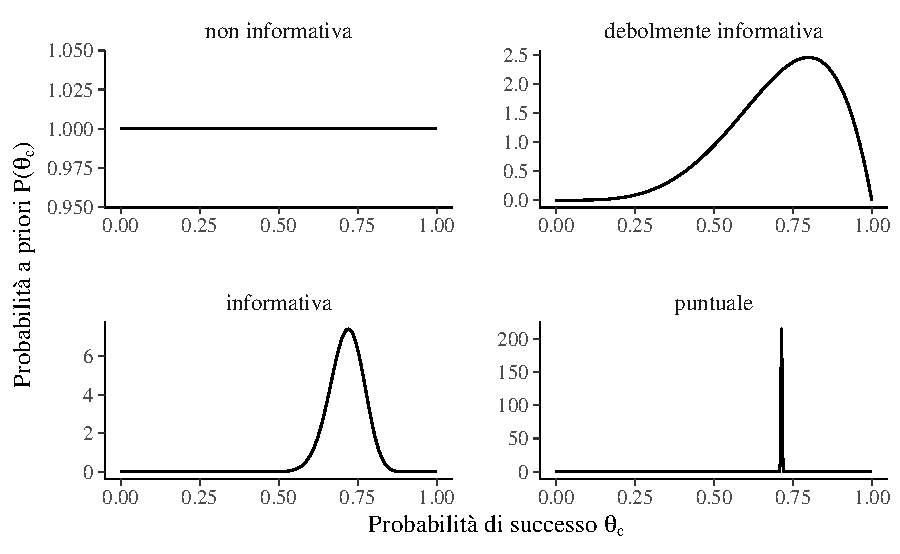
\includegraphics{025_intro_bayes_files/figure-latex/ch-03-02-models-types-of-priors-1} 

}

\caption{Esempi di distribuzioni a priori per il parametro $\theta_c$ nel Modello Binomiale.}\label{fig:ch-03-02-models-types-of-priors}
\end{figure}

\hypertarget{scelta-della-distribuzione-a-priori}{%
\subsection{Scelta della distribuzione a priori}\label{scelta-della-distribuzione-a-priori}}

La selezione delle distribuzioni a priori è stata spesso vista come una delle scelte più importanti che un ricercatore fa quando implementa un modello bayesiano in quanto può avere un impatto sostanziale sui risultati finali. La soggettività delle distribuzioni a priori è evidenziata dai critici come un potenziale svantaggio dei metodi bayesiani. A questa critica, \citet{vandeSchoot2021modelling} rispondono dicendo che, al di là della scelta delle distribuzioni a priori, ci sono molti elementi del processo di inferenza statistica che sono soggettivi, ovvero la scelta del modello statistico e le ipotesi sulla distribuzione degli errori. In secondo luogo, \citet{vandeSchoot2021modelling} notano come le distribuzioni a priori svolgono due importanti ruoli statistici: quello della ``regolarizzazione della stima'', ovvero, il processo che porta ad indebolire l'influenza indebita di osservazioni estreme, e quello del miglioramento dell'efficienza della stima, ovvero, la facilitazione dei processi di calcolo numerico di stima della distribuzione a posteriori. L'effetto della distribuzione a priori sulla distribuzione a posteriori verrà discusso nel Capitolo \ref{chapter-balance}.

\hypertarget{verosim-marginale}{%
\section{Verosimiglianza marginale}\label{verosim-marginale}}

Al denominatore della regola di Bayes abbiamo la verosimiglianza marginale \(p(y)\). Tale denominatore è espresso nei termini di un integrale che, tranne in pochi casi particolari, non ha una soluzione analitica.

\hypertarget{la-distribuzione-a-posteriori}{%
\section{La distribuzione a posteriori}\label{la-distribuzione-a-posteriori}}

Ci sono due metodi principali per calcolare la distribuzione a posteriori \(p(\theta \mid y)\):

\begin{itemize}
\tightlist
\item
  una precisa derivazione matematica formulata nei termini della distribuzione a priori coniugata alla distribuzione a posteriori (si veda il Capitolo \ref{chapter-distr-coniugate}); tale procedura però ha un'applicabilità molto limitata;
\item
  un metodo approssimato, molto facile da utilizzare in pratica, che dipende da metodi Monte Carlo basati su Catena di Markov (MCMC).
\end{itemize}

Una volta calcolata la distribuzione a posteriori dobbiamo riassumerla in qualche modo. Questo problema verrà discusso nel Capitolo \ref{chapter-sintesi-distr-post}.

\hypertarget{considerazioni-conclusive}{%
\section*{Considerazioni conclusive}\label{considerazioni-conclusive}}
\addcontentsline{toc}{section}{Considerazioni conclusive}

In base all'approccio bayesiano, invece di dire che il parametro di interesse di un modello statistico ha un valore vero ma sconosciuto, diciamo che, prima di eseguire l'esperimento, è possibile assegnare una distribuzione di probabilità, che chiamano stato di credenza, a quello che è il vero valore del parametro. Questa distribuzione a priori può essere nota (per esempio, sappiamo che la distribuzione dei punteggi del QI è normale con media 100 e deviazione standard 15) o può essere del tutto arbitraria. L'inferenza bayesiana procede poi nel modo seguente: si raccolgono alcuni dati e si calcola la probabilità dei possibili valori del parametro alla luce dei dati osservati e delle credenze a priori. Questa nuova distribuzione di probabilità è chiamata ``distribuzione a posteriori'' e riassume l'incertezza dell'inferenza.

  \bibliography{refs.bib,book.bib,packages.bib}

\end{document}
